\chapter{Tổng quan lý thuyết và nghiên cứu liên quan}

\section{Các khái niệm cơ bản}
\subsection{Trục tích hợp dữ liệu}
Trong bối cảnh công nghệ số hiện đại, các tổ chức, doanh nghiệp phải đối mặt với thách thức quản lý và xử lý lượng dữ liệu khổng lồ từ nhiều nguồn phân tán. Sự phức tạp này đòi hỏi một giải pháp kiến trúc có khả năng tập trung hóa và điều phối luồng dữ liệu một cách hiệu quả. Nền tảng đảm nhận nhiệm vụ này chính là Trục tích hợp dữ liệu.

Trục tích hợp dữ liệu hoạt động như một điểm trung gian, kết nối các hệ thống nguồn và các ứng dụng tiêu thụ dữ liệu. Thay vì tạo ra các kết nối point-to-point phức tạp, trục tích hợp dữ liệu đơn giản hóa kiến trúc bằng cách cung cấp một điểm trao đổi dữ liệu duy nhất, giúp việc lưu trữ, xử lý và đồng bộ hóa thông tin trở nên dễ dàng và nhất quán hơn. Trong môi trường đại học, nơi dữ liệu ở nhiều nơi, việc áp dụng một trục tích hợp dữ liệu càng trở nên cấp thiết để đảm bảo thông tin được xuyên suốt và chính xác.

Theo định nghĩa của Informatica, một trong những công ty hàng đầu về quản lý dữ liệu:
\begin{quote}
"Trung tâm tích hợp dữ liệu đóng vai trò là nền tảng tập trung, cho phép các tổ chức tích hợp, quản lý và quản trị dữ liệu một cách liền mạch trên nhiều hệ thống và ứng dụng phân tích khác nhau. Hoạt động như một kênh dẫn dữ liệu, trung tâm tích hợp dữ liệu hợp nhất thông tin từ các nguồn khác nhau, chẳng hạn như cơ sở dữ liệu, dịch vụ đám mây và hệ thống cũ, tạo điều kiện thuận lợi cho việc trao đổi và đồng bộ hóa dữ liệu hiệu quả. Trung tâm này hoạt động như một đơn vị trung gian, đảm bảo dữ liệu được truyền tải thông suốt giữa các hệ thống, đồng thời cung cấp các khả năng về chất lượng dữ liệu, bảo mật và quản trị." \cite{informatica:whatisdih}
\end{quote}

Trong khi đó, AWS định nghĩa khái niệm "Tích hợp dữ liệu" ở phạm vi rộng hơn, nhấn mạnh đến mục tiêu cuối cùng là tạo ra giá trị từ dữ liệu:
\begin{quote}
"Tích hợp dữ liệu là quá trình đạt được quyền truy cập và phân phối nhất quán cho tất cả các loại dữ liệu trong doanh nghiệp. [...] Tích hợp dữ liệu liên quan đến các kỹ thuật, công cụ và phương thức về kiến trúc nhằm hợp nhất các nguồn dữ liệu khác nhau cho hoạt động phân tích. Do đó, các tổ chức có thể xem đầy đủ dữ liệu của họ để biết thông tin chuyên sâu và nghiệp vụ thông minh có giá trị cao." \cite{aws:whatisdi}
\end{quote}

Từ hai định nghĩa trên, có thể thấy Trục tích hợp dữ liệu là một kiến trúc cụ thể để hiện thực hóa việc tích hợp dữ liệu. Nó không chỉ là công cụ truyền tải mà còn là một nền tảng quản trị tập trung. Các nhiệm vụ chính của một trục tích hợp dữ liệu bao gồm:

\begin{itemize}
    \item \textbf{Thu thập và phân phối dữ liệu:} Tiếp nhận dữ liệu từ các hệ thống nguồn và phân phối đến các hệ thống đích theo mô hình publish/subscribe (đăng ký/xuất bản) \cite{microsoft:pubsub, confluent:pubsub}.
    \item \textbf{Điều phối và định tuyến:} Tổng hợp và chuyển tiếp dữ liệu đến các hệ thống hoặc ứng dụng cần thiết, đồng thời áp dụng các quy tắc phân quyền để đảm bảo an toàn thông tin.
    \item \textbf{Đảm bảo chất lượng dữ liệu:} Kiểm tra tính hợp lệ, nhất quán và tuân thủ các tiêu chuẩn định sẵn của dữ liệu. Dữ liệu không đạt chuẩn có thể bị từ chối hoặc chuyển vào một quy trình làm sạch riêng, nhằm duy trì sự toàn vẹn cho toàn hệ thống.
    \item \textbf{Giám sát và ghi nhật ký:} Theo dõi toàn bộ quá trình trao đổi dữ liệu, ghi lại các sự kiện quan trọng để phục vụ cho việc kiểm tra, gỡ lỗi và phân tích hiệu suất.
    \item \textbf{Lập lịch:} Tự động hóa việc thực thi các tác vụ tích hợp dữ liệu theo những khoảng thời gian được định trước.
\end{itemize}

Việc triển khai một trục tích hợp dữ liệu mang lại nhiều vai trò và lợi ích quan trọng, đặc biệt với các hệ thống phức tạp, đa nguồn dữ liệu:

\begin{itemize}
    \item \textbf{Giảm sự phức tạp của hệ thống:} Bằng cách thay thế mạng lưới kết nối point-to-point chằng chịt, hệ thống trở nên dễ quản lý, bảo trì và phát triển hơn.
    \item \textbf{Tăng cường tính nhất quán của dữ liệu:} Đảm bảo rằng tất cả các ứng dụng đều truy cập vào cùng một nguồn dữ liệu đã được xác thực và đồng bộ, loại bỏ tình trạng xung đột và sai lệch thông tin \cite{microsoft:pubsub, gartner:data_consistency}.
    \item \textbf{Tăng tính linh hoạt và khả năng mở rộng:} Khi một hệ thống mới cần tham gia vào mạng lưới, chỉ cần kết nối nó với trục trung tâm thay vì phải xây dựng kết nối riêng lẻ tới tất cả các hệ thống khác \cite{confluent:pubsub}.
    \item \textbf{Nền tảng cho phân tích dữ liệu:} Trục tích hợp dữ liệu cung cấp dữ liệu sạch, nhất quán và tập trung, tạo điều kiện lý tưởng cho các hoạt động phân tích kinh doanh, học máy và hỗ trợ ra quyết định \cite{informatica:whatisdih,ibm:bi_from_di}.
\end{itemize}

Tóm lại, trục tích hợp dữ liệu là một thành phần kiến trúc chiến lược, đóng vai trò trung gian điều phối luồng thông tin giữa các nguồn dữ liệu và các hệ thống tiêu thụ, qua đó đảm bảo sự ổn định, nhất quán và linh hoạt cho toàn bộ hệ sinh thái dữ liệu của một tổ chức.

\subsection{OLTP và OLAP}
Trong lĩnh vực xử lý dữ liệu, hai loại hệ thống chính thường được nhắc đến là OLTP và OLAP, phục vụ cho hai mục đích hoàn toàn khác nhau.

\subsubsection{OLTP (Online Transaction Processing)}
OLTP, viết tắt của Xử lý giao dịch trực tuyến (Online Transaction Processing), ám chỉ các hệ thống được thiết kế để quản lý và xử lý một khối lượng lớn các giao dịch ngắn, diễn ra trong thời gian thực. Các giao dịch này thường là các thao tác cơ sở dữ liệu cơ bản như thêm (INSERT), sửa (UPDATE), và xóa (DELETE).

Ví dụ điển hình là hệ thống của máy ATM, hệ thống đặt vé máy bay, hay hệ thống quản lý sinh viên của một trường đại học khi sinh viên đăng ký môn học. Mục tiêu chính của hệ thống OLTP là đảm bảo tính sẵn sàng cao, tốc độ xử lý nhanh, khả năng chịu tải đồng thời lớn và tính toàn vẹn dữ liệu (thông qua các thuộc tính ACID - Atomicity, Consistency, Isolation, Durability) \cite{microsoft:oltp}. Do đó, cơ sở dữ liệu của OLTP thường được thiết kế theo mô hình quan hệ và được chuẩn hóa cao để tối ưu cho các thao tác ghi và cập nhật.

\subsubsection{OLAP (Online Analytical Processing)}
Ngược lại với OLTP, OLAP (Xử lý phân tích trực tuyến - Online Analytical Processing) là các hệ thống được tối ưu cho việc thực hiện các truy vấn phân tích phức tạp trên một lượng lớn dữ liệu. Thay vì xử lý các giao dịch hàng ngày, mục tiêu của OLAP là hỗ trợ việc ra quyết định kinh doanh, phân tích xu hướng và khai phá dữ liệu \cite{pareek2007business}.

Hệ thống OLAP thường hoạt động trên các Kho dữ liệu, chứa dữ liệu lịch sử được tổng hợp từ nhiều hệ thống OLTP khác nhau. Nền tảng của OLAP là mô hình dữ liệu đa chiều, thường được hình dung như một khối dữ liệu. Theo Jiawei Han và các cộng sự, mô hình này cho phép dữ liệu được tổ chức theo nhiều chiều và mỗi chiều lại chứa nhiều cấp độ trừu tượng khác nhau, giúp người dùng có thể linh hoạt xem xét dữ liệu từ nhiều góc độ \cite{han2011datamining}.

Các thao tác phân tích điển hình trên một khối dữ liệu OLAP bao gồm \cite{han2011datamining}:
\begin{itemize}
    \item \textbf{Roll-up (Tổng hợp):} Thao tác tổng hợp dữ liệu bằng cách đi lên các cấp cao hơn trong một hệ thống phân cấp của chiều dữ liệu.
    \item \textbf{Drill-down (Chi tiết hóa):} Thao tác ngược lại với roll-up, đi từ dữ liệu ít chi tiết đến dữ liệu chi tiết hơn.
    \item \textbf{Slice (Cắt lát):} Chọn một giá trị trên một chiều để tạo ra một khối dữ liệu con.
    \item \textbf{Dice (Cắt khối):} Chọn một dải giá trị trên hai hoặc nhiều chiều để tạo ra một khối dữ liệu con.
\end{itemize}

\subsubsection{So sánh OLTP và OLAP}
Sự khác biệt cơ bản giữa hai hệ thống có thể được tóm tắt trong bảng dưới đây.
\begin{table}[ht!]
    \centering
    \begin{tabular}{|l|p{5.5cm}|p{5.5cm}|}
        \hline
        \textbf{Tiêu chí} & \textbf{OLTP} & \textbf{OLAP} \\
        \hline
        \textbf{Mục tiêu chính} & Quản lý các hoạt động nghiệp vụ hàng ngày & Hỗ trợ ra quyết định và phân tích chiến lược \\
        \hline
        \textbf{Loại thao tác} & Các giao dịch nhỏ, nhanh (INSERT, UPDATE, DELETE) & Các truy vấn phức tạp, tổng hợp (SELECT, GROUP BY) \\
        \hline
        \textbf{Tối ưu cho} & Thao tác ghi (Write-intensive) & Thao tác đọc (Read-intensive) \\
        \hline
        \textbf{Nguồn dữ liệu} & Dữ liệu hoạt động, thời gian thực & Dữ liệu lịch sử, được tổng hợp từ nhiều nguồn \\
        \hline
        \textbf{Cấu trúc CSDL} & Chuẩn hóa cao (Normalized - ER Model) & Phi chuẩn hóa (Denormalized - Star/Snowflake Schema) \\
        \hline
        \textbf{Đối tượng sử dụng} & Nhân viên nghiệp vụ, người dùng cuối & Nhà phân tích dữ liệu, nhà quản lý \\
        \hline
    \end{tabular}
    \caption{So sánh sự khác biệt giữa OLTP và OLAP}
    \label{tab:oltp_olap_comparison}
\end{table}

\textbf{Áp dụng cho Trục tích hợp dữ liệu:} 
Trong bối cảnh của một trường đại học, hệ thống quản lý sinh viên (nơi sinh viên đăng ký môn học, phòng đào tạo nhập điểm) là một hệ thống OLTP điển hình. Trong khi đó, một hệ thống báo cáo cho ban giám hiệu để phân tích xu hướng tuyển sinh qua các năm, tỷ lệ tốt nghiệp theo từng khoa, hoặc hiệu quả sử dụng phòng học sẽ là một hệ thống OLAP, lấy dữ liệu từ hệ thống quản lý sinh viên và các nguồn khác. Trong kiến trúc của đề tài, Trục tích hợp đóng vai trò cầu nối. Dữ liệu thu thập từ các nguồn được trục tích hợp thu thập và lưu trữ vào cơ sở dữ liệu trung tâm. Cơ sở dữ liệu này cần cân bằng giữa khả năng ghi, từ quá trình đồng bộ và khả năng đọc. Do đó, thiết kế CSDL của trục sẽ thiên hướng về hỗ trợ dữ liệu tích hợp từ nhiều nguồn OLTP nhưng vẫn đảm bảo cấu trúc nhất quán để phục vụ các truy vấn khai thác nhanh chóng.

\subsection{ETL và ELT}
Khi dữ liệu được thu thập từ nhiều hệ thống nguồn (như các hệ thống OLTP), chúng thường ở dạng thô, không đồng nhất về cấu trúc và định dạng. Để có thể sử dụng dữ liệu này cho mục đích phân tích trong một kho dữ liệu, cần có một quy trình để xử lý và hợp nhất chúng. ETL và ELT là hai quy trình phổ biến nhất để thực hiện nhiệm vụ này.

\subsubsection{Quy trình ETL (Extract - Transform - Load)}
ETL là viết tắt của \textbf{Extract (Trích xuất), Transform (Biến đổi), Load (Nạp)}. Đây là một quy trình truyền thống và được sử dụng rộng rãi, bao gồm ba giai đoạn chính \cite{wiki:etl}:
\begin{enumerate}
    \item \textbf{Extract:} Dữ liệu được trích xuất từ các hệ thống nguồn đa dạng như cơ sở dữ liệu quan hệ (SQL), cơ sở dữ liệu NoSQL, các file phẳng (CSV, XML, JSON), hoặc các API. Ở giai đoạn này, dữ liệu được lấy ra khỏi nguồn và đưa vào một khu vực tạm gọi là Staging Area.
    
    \item \textbf{Transform:} Đây là giai đoạn quan trọng nhất, nơi dữ liệu thô được xử lý để đảm bảo chất lượng và tính nhất quán. Các tác vụ biến đổi phổ biến bao gồm:
    \begin{itemize}
        \item \textbf{Làm sạch:} Sửa lỗi chính tả, xử lý các giá trị bị thiếu (null), loại bỏ dữ liệu trùng lặp.
        \item \textbf{Chuẩn hóa:} Đưa các trường dữ liệu về một định dạng chung. Ví dụ, chuyển đổi trường mã sinh viên sid từ hệ thống A và student\_id từ hệ thống B thành một trường duy nhất là MaSinhVien trong hệ thống đích.
        \item \textbf{Tích hợp:} Kết hợp dữ liệu từ nhiều nguồn khác nhau. Ví dụ, nối thông tin học tập của sinh viên với thông tin học phí của họ.
        \item \textbf{Tổng hợp:} Tính toán các giá trị tổng hợp như tổng, trung bình, v.v.
    \end{itemize}
    
    \item \textbf{Load:} Sau khi đã được biến đổi, dữ liệu sạch và có cấu trúc sẽ được nạp vào hệ thống đích, thường là một Kho dữ liệu (Data Warehouse) hoặc một Data Mart để phục vụ cho các hệ thống OLAP và Business Intelligence.
\end{enumerate}

\begin{figure}[h!]
    \centering
    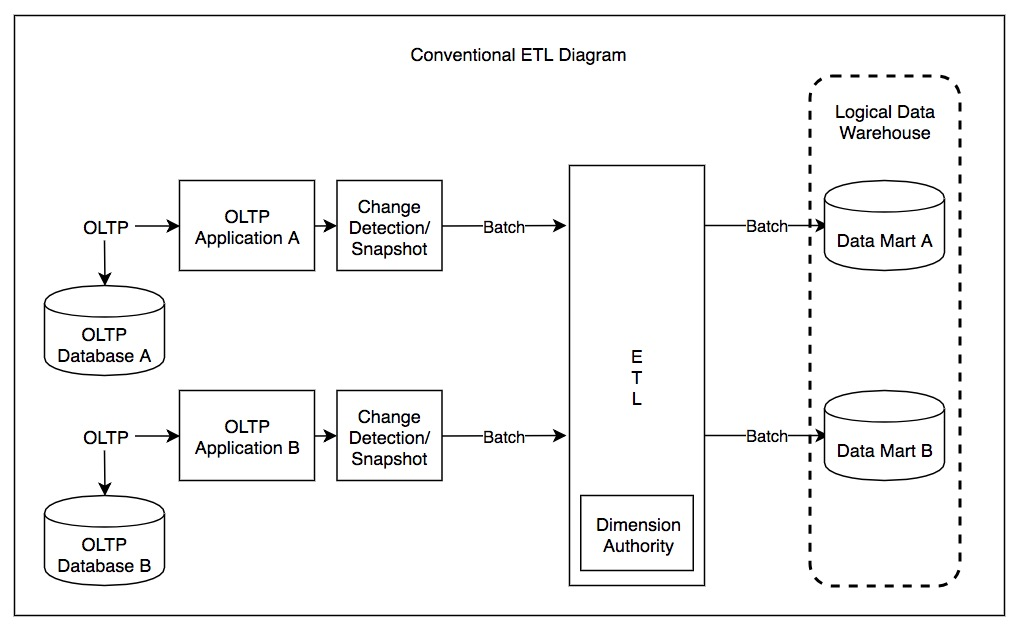
\includegraphics[width=0.8\textwidth]{graphics/etl_oltp.jpg}
    \caption{Mô hình quy trình ETL điển hình, trích xuất dữ liệu từ các hệ thống nguồn (OLTP) để nạp vào Kho dữ liệu (Data Warehouse) \cite{wiki:etl}}
    \label{fig:etl_process}
\end{figure}

\subsubsection{Quy trình ELT (Extract - Load - Transform)}
Với sự phát triển của các kho dữ liệu trên nền tảng đám mây có khả năng xử lý song song cực lớn như Google BigQuery, Amazon Redshift, hay Snowflake, một quy trình mới đã ra đời là ELT.

Trong mô hình ELT, thứ tự các bước được thay đổi: Dữ liệu được trích xuất từ nguồn và được \textbf{nạp (Load)} ngay lập tức vào kho dữ liệu ở dạng thô. Sau đó, quá trình \textbf{biến đổi (Transform)} sẽ được thực hiện trực tiếp bên trong kho dữ liệu bằng cách tận dụng năng lực tính toán mạnh mẽ của nó.

\begin{table}[h!]
    \centering
    \begin{tabular}{|l|p{5.5cm}|p{5.5cm}|}
        \hline
        \textbf{Tiêu chí} & \textbf{ETL (Truyền thống)} & \textbf{ELT (Hiện đại)} \\
        \hline
        \textbf{Thứ tự} & Extract \(\rightarrow\) Transform \(\rightarrow\) Load & Extract \(\rightarrow\) Load \(\rightarrow\) Transform \\
        \hline
        \textbf{Nơi biến đổi} & Trên một server trung gian (Staging Server) & Trực tiếp trong Kho dữ liệu đích \\
        \hline
        \textbf{Thời gian nạp} & Chậm hơn, vì phải chờ biến đổi xong & Rất nhanh, nạp dữ liệu thô ngay lập tức \\
        \hline
        \textbf{Lưu trữ} & Chỉ lưu trữ dữ liệu đã biến đổi & Lưu trữ cả dữ liệu thô và dữ liệu đã biến đổi \\
        \hline
        \textbf{Phù hợp với} & Dữ liệu có cấu trúc, quy tắc biến đổi rõ ràng & Dữ liệu lớn (Big Data), dữ liệu phi cấu trúc, cần sự linh hoạt \\
        \hline
    \end{tabular}
    \caption{So sánh giữa quy trình ETL và ELT}
    \label{tab:etl_vs_elt}
\end{table}

\subsubsection{Ứng dụng trong Trục tích hợp}

Mặc dù quy trình ETL/ELT là cần thiết, trong bối cảnh trường đại học, dữ liệu thường phân tán ở các hệ thống quản lý độc lập với cấu trúc dữ liệu và quy ước định danh khác nhau. Nếu hệ thống trục tích hợp phải tự mình xử lý từng định dạng riêng biệt, việc mở rộng và bảo trì sẽ trở nên rất phức tạp.

Thay vì vậy, một cách tiếp cận hiệu quả hơn là định nghĩa một mô hình dữ liệu chuẩn cho toàn trường. Trục tích hợp sẽ công bố các chuẩn dữ liệu, định dạng tệp, hoặc API đầu vào theo mô hình này. Mỗi phòng ban khi gửi dữ liệu lên trục tích hợp phải tuân thủ định dạng chuẩn đó. 

Dữ liệu gửi đến trục tích hợp sẽ trải qua các bước:
\begin{itemize}
    \item \textbf{Extract:} Tiếp nhận dữ liệu được gửi đến từ các hệ thống nguồn (qua API, file upload, hoặc message queue).
    \item \textbf{Validate:} Kiểm tra cấu trúc, kiểu dữ liệu, và giá trị theo bộ tiêu chuẩn đã được định nghĩa (ví dụ: \textit{MaSV} phải là chuỗi 8 ký tự, ngày sinh phải hợp lệ, mã khoa phải tồn tại trong danh mục).
    \item \textbf{Transform \& Load:} Nếu dữ liệu hợp lệ, trục tích hợp sẽ chuyển đổi về mô hình dữ liệu chuẩn nội bộ và nạp vào kho dữ liệu dùng chung.
\end{itemize}

Với cách tiếp cận này, hệ thống trục tích hợp không cần biết chi tiết về cách từng đơn vị nội bộ tổ chức dữ liệu, mà chỉ cần đảm bảo mọi dữ liệu đầu vào tuân thủ chuẩn thống nhất. Điều này giúp giảm độ phức tạp, đảm bảo tính nhất quán, và tăng khả năng mở rộng của toàn hệ thống.

\section{Các kiến trúc tích hợp dữ liệu}
Việc lựa chọn một kiến trúc tích hợp phù hợp là yếu tố nền tảng quyết định sự thành công, khả năng mở rộng và bảo trì của một hệ thống. Dưới đây là phân tích về các mô hình kiến trúc phổ biến, từ truyền thống đến hiện đại.

\subsection{Kiến trúc điểm-nối-điểm (Point-to-Point - P2P)}
\begin{figure}[h!]
    \centering
    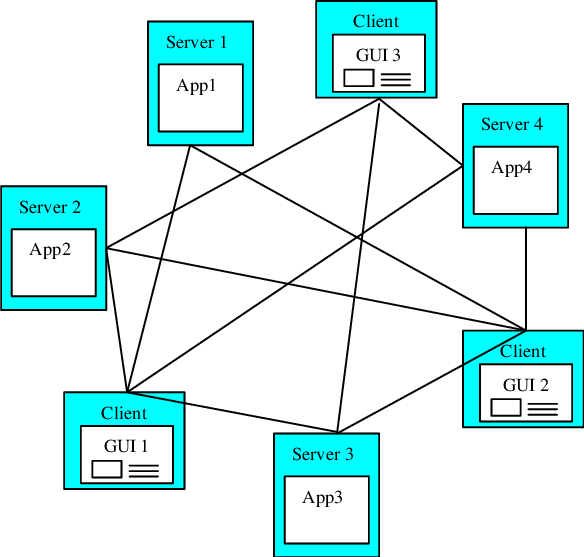
\includegraphics[width=0.8\textwidth]{graphics/p2p-architect.png}
    \caption{Kiến trúc Point-to-point \cite{inproceedings}}
    \label{fig:p2p_architect} 
\end{figure}
\begin{itemize}
    \item \textbf{Mô tả:} Đây là kiến trúc cơ bản nhất, trong đó mỗi hệ thống được kết nối trực tiếp với một hệ thống khác khi có nhu cầu trao đổi dữ liệu. Nếu hệ thống A cần dữ liệu từ hệ thống B, một kết nối riêng lẻ sẽ được thiết lập giữa chúng.
    \item \textbf{Ưu điểm:} Triển khai nhanh chóng và đơn giản cho các kịch bản có quy mô rất nhỏ (chỉ từ 2 đến 3 hệ thống).
    \item \textbf{Nhược điểm:} Khi số lượng hệ thống tăng lên, số lượng kết nối sẽ tăng theo cấp số nhân, tuân theo công thức \(n(n-1)/2\), với \(n\) là số hệ thống. Điều này nhanh chóng tạo ra một cấu trúc phức tạp, khó quản lý, khó theo dõi và bảo trì, thường được gọi là "kiến trúc spaghetti".
\end{itemize}

\subsection{Kiến trúc trục và nan hoa (Hub-and-Spoke)}
\begin{itemize}
    \item \textbf{Mô tả:} Đây là mô hình kinh điển của một trục tích hợp dữ liệu. Một Hub (trục) trung tâm được thiết lập, và tất cả các hệ thống con (Spokes - nan hoa) đều kết nối vào Hub này thay vì kết nối trực tiếp với nhau. Hub chịu trách nhiệm tiếp nhận, biến đổi, và định tuyến dữ liệu giữa các nan hoa.
    \item \textbf{Ưu điểm:} Cung cấp khả năng quản lý tập trung; giảm thiểu đáng kể số lượng kết nối so với P2P; dễ dàng thêm hoặc bớt các hệ thống con mà không ảnh hưởng đến toàn bộ mạng lưới.
    \item \textbf{Nhược điểm:} Hub trung tâm có nguy cơ trở thành điểm nghẽn cổ chai (single point of failure and bottleneck). Nếu Hub gặp sự cố, toàn bộ luồng dữ liệu trong hệ thống sẽ bị gián đoạn.
\end{itemize}

\subsection{Kiến trúc bus dịch vụ doanh nghiệp (Enterprise Service Bus - ESB)}
\begin{figure}[h!]
    \centering
    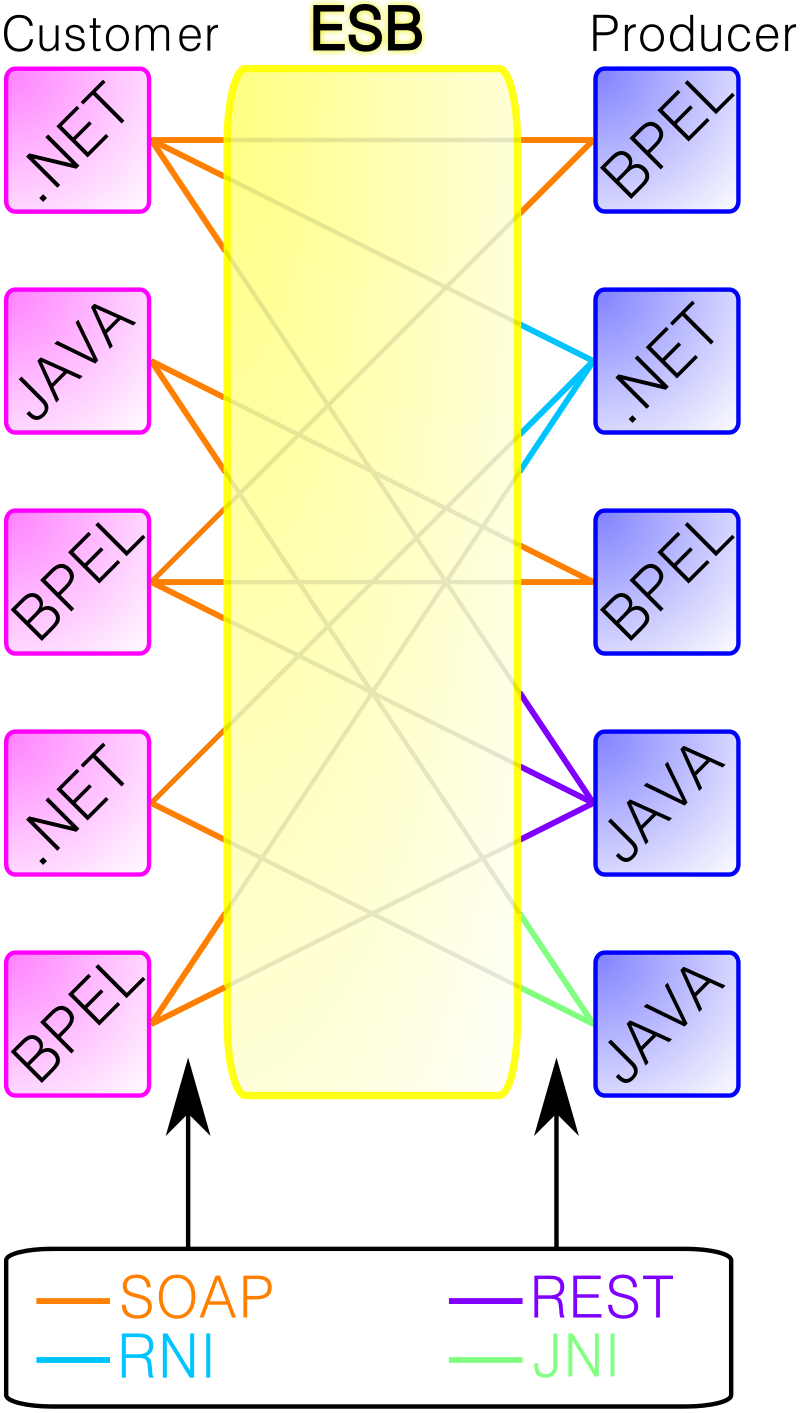
\includegraphics[width=0.5\textwidth]{graphics/esb.png}
    \caption{Kiến trúc Enterprise Service Bus \cite{wiki:esb}}
    \label{fig:esb_architect} 
\end{figure}

\begin{itemize}
    \item \textbf{Mô tả:} ESB có thể được xem là một sự tiến hóa của mô hình Hub-and-Spoke. Nó hoạt động như một nền tảng trung gian mà các ứng dụng và dịch vụ có thể kết nối vào. ESB không chỉ đơn thuần truyền tải dữ liệu mà còn cung cấp một loạt các dịch vụ giá trị gia tăng như: điều phối quy trình nghiệp vụ, chuyển đổi giao thức, định tuyến thông điệp thông minh, và quản lý bảo mật.
    \item \textbf{Ưu điểm:} Rất mạnh mẽ và linh hoạt, có khả năng xử lý các quy trình nghiệp vụ phức tạp, phù hợp cho các doanh nghiệp lớn với hệ sinh thái ứng dụng đa dạng.
    \item \textbf{Nhược điểm:} Việc triển khai và vận hành một hệ thống ESB thường rất phức tạp và tốn kém, đòi hỏi chuyên môn kỹ thuật cao.
\end{itemize}

\subsection{Kiến trúc kết nối dựa trên API (API-led Connectivity)}
\begin{figure}[h!]
    \centering
    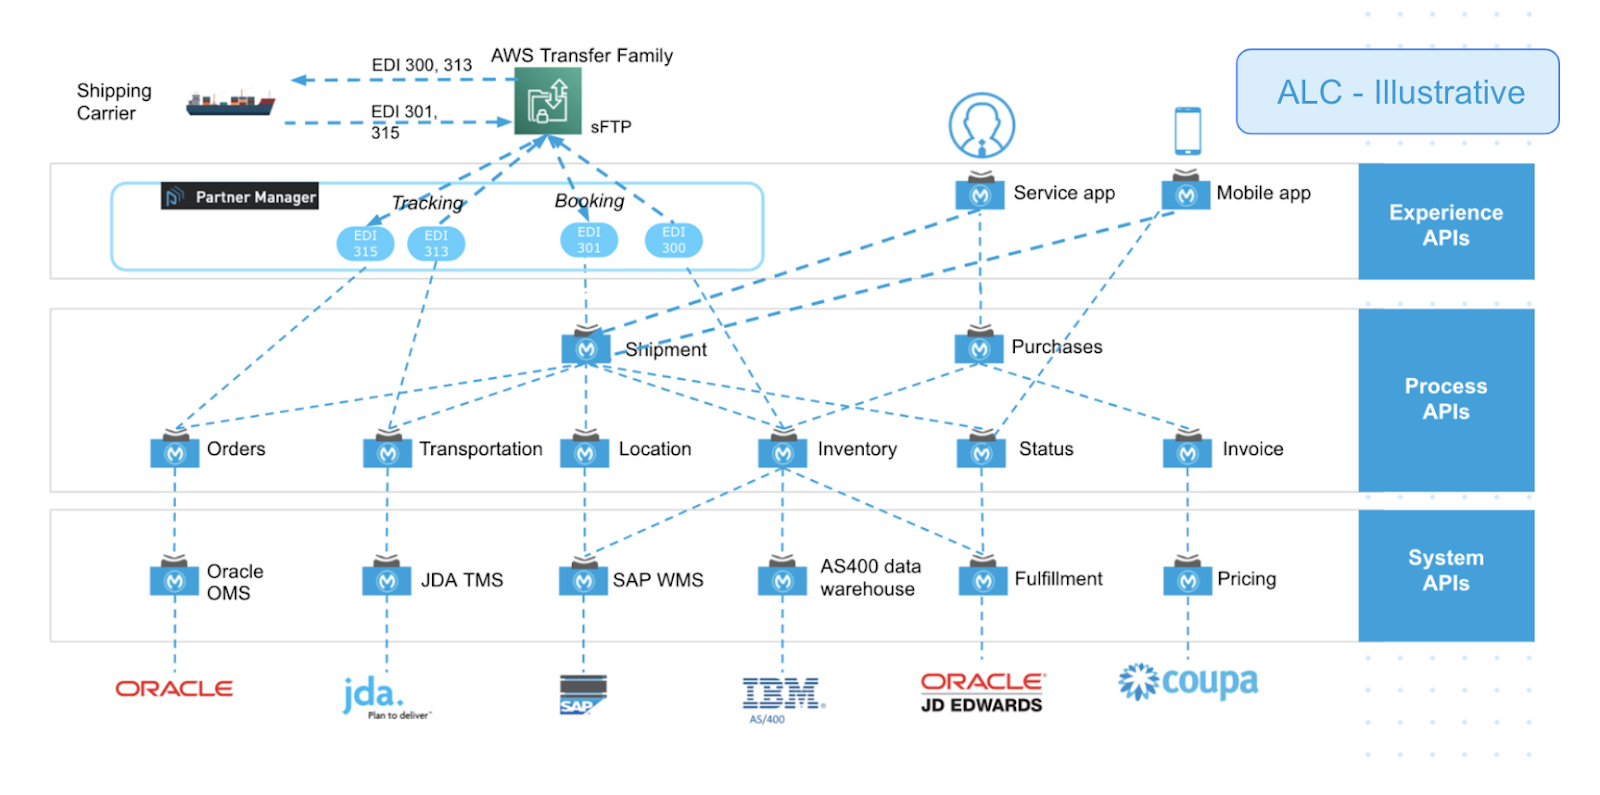
\includegraphics[width=1.0\textwidth]{graphics/api-led.png}
    \caption{Minh hoạ cho kiến trúc API-led Connectivity\cite{mulesoft:apiled}}
    \label{fig:api_led_architect} 
\end{figure}
\begin{itemize}
    \item \textbf{Mô tả:} Đây là một phương pháp tiếp cận hiện đại, tập trung vào việc thiết kế và xây dựng các Giao diện lập trình ứng dụng (API) có khả năng tái sử dụng cao. Thay vì xây dựng một hệ thống trung tâm nguyên khối, kiến trúc này phân lớp các API thành ba tầng riêng biệt \cite{mulesoft:apiled}:
    \begin{itemize}
        \item \textbf{System APIs (API Hệ thống):} Lớp dưới cùng, có nhiệm vụ trừu tượng hóa (abstract) và mở khóa dữ liệu từ các hệ thống lõi (ví dụ: CSDL sinh viên, hệ thống tài chính). Các API này chỉ tập trung vào việc cung cấp dữ liệu thô một cách an toàn và nhất quán.
        \item \textbf{Process APIs (API Quy trình):} Lớp giữa, thực hiện việc điều phối và kết hợp dữ liệu từ nhiều System API để tạo ra các chức năng nghiệp vụ cụ thể. Ví dụ, một API "Tổng hợp thông tin sinh viên" sẽ gọi đến System API từ hệ thống đào tạo, tài chính và ký túc xá để trả về một bản ghi hoàn chỉnh.
        \item \textbf{Experience APIs (API Trải nghiệm):} Lớp trên cùng, được thiết kế để phục vụ cho một kênh hoặc một trải nghiệm người dùng cuối cụ thể, ví dụ: API cho ứng dụng di động của sinh viên, API cho cổng thông tin dành cho giảng viên.
    \end{itemize}
    \item \textbf{Ưu điểm:} Thúc đẩy tính linh hoạt, khả năng tái sử dụng và tốc độ phát triển; phù hợp với các kiến trúc hiện đại như Microservices; cho phép phát triển và mở rộng một cách phân tán.
\end{itemize}

\subsection{So sánh và lựa chọn kiến trúc cho bối cảnh đại học}
Sau khi phân tích các mô hình, việc lựa chọn kiến trúc API-led Connectivity được xem là phù hợp nhất cho bối cảnh của một trường đại học hiện đại. Dưới đây là các lập luận chi tiết.

\subsubsection{Những hạn chế của kiến trúc truyền thống}
Các mô hình như Hub-and-Spoke và ESB, mặc dù có giá trị trong nhiều ngữ cảnh, lại bộc lộ những nhược điểm đáng kể khi áp dụng vào một môi trường đòi hỏi sự linh hoạt và đổi mới nhanh như trường đại học:
\begin{itemize}
    \item \textbf{Tạo ra kiến trúc trung tâm nguyên khối (Monolithic Hub):} Toàn bộ logic tích hợp (biến đổi, định tuyến) bị tập trung vào một Hub hoặc Bus duy nhất. Điều này làm cho thành phần trung tâm trở nên phức tạp, khó phát triển, bảo trì và nâng cấp.
    \item \textbf{Điểm nghẽn và rủi ro hệ thống:} Vì mọi luồng dữ liệu đều phải đi qua điểm trung tâm, hệ thống rất dễ bị quá tải khi lưu lượng tăng cao. Sự cố tại trung tâm sẽ làm tê liệt toàn bộ hệ thống.
    \item \textbf{Hạn chế tính linh hoạt và khả năng đáp ứng nhanh:} Khi có nhu cầu phát triển một ứng dụng mới (ví dụ: ứng dụng cho tuần lễ hướng nghiệp), các nhóm phát triển phải phụ thuộc vào đội ngũ quản lý hệ thống trung tâm để xây dựng các kết nối và logic mới. Quá trình này thường chậm chạp và cản trở sự đổi mới.
    \item \textbf{Sự phức tạp và chi phí của ESB:} Một hệ thống ESB đầy đủ chức năng thường quá cồng kềnh và tốn kém, vượt quá nhu cầu và quy mô của hầu hết các trường đại học, đồng thời có nguy cơ phụ thuộc vào nhà cung cấp.
\end{itemize}

\subsubsection{Lý do lựa chọn kiến trúc kết nối dựa trên API}
Kiến trúc kết nối dựa trên API giải quyết trực tiếp các vấn đề nêu trên và mang lại nhiều lợi ích chiến lược:
\begin{itemize}
    \item \textbf{Thúc đẩy tái sử dụng và tăng tốc độ phát triển:} Thay vì xây dựng các kết nối dùng một lần, kiến trúc này tạo ra một danh mục các API có thể được tái sử dụng trên nhiều dự án. Ví dụ, System API "Thông tin sinh viên" sau khi được xây dựng có thể phục vụ cho cả ứng dụng di động, cổng thông tin giảng viên, và hệ thống thư viện mà không cần phát triển lại, giúp giảm thời gian triển khai các sáng kiến mới một cách đáng kể.
    \item \textbf{Phân tán và dễ dàng mở rộng:} Logic tích hợp không còn bị dồn vào một điểm. Mỗi API là một thành phần độc lập, có thể được phát triển, triển khai và mở rộng riêng lẻ bởi các nhóm khác nhau. Điều này hoàn toàn phù hợp với triết lý của kiến trúc Microservices.
    \item \textbf{Tăng cường bảo mật và quản trị:} Mỗi API hoạt động như một cổng kiểm soát (gateway). Thông qua một API Gateway, nhà trường có thể dễ dàng áp dụng các chính sách bảo mật, giới hạn tần suất truy cập, và kiểm soát quyền truy cập dữ liệu cho từng ứng dụng một cách chi tiết và an toàn.
    \item \textbf{Sẵn sàng cho hệ sinh thái mở và tương lai:} Kiến trúc này giúp trường đại học không chỉ tích hợp hiệu quả các hệ thống nội bộ mà còn dễ dàng kết nối với các hệ thống bên ngoài (như hệ thống của Bộ Giáo dục và Đào tạo), các đối tác doanh nghiệp, hoặc tích hợp các công nghệ mới (IoT, AI/ML) bằng cách tạo ra các API mới mà không làm xáo trộn kiến trúc hiện có.
\end{itemize}